\documentclass[11pt, a4paper]{article} % Formato

% Language and font encodings
\usepackage[spanish]{babel}
\usepackage[utf8]{inputenc}
\usepackage[T1]{fontenc}
\usepackage{times} % Times New Roman

%% Sets page size and margins
\usepackage[margin=2.5cm, includefoot]{geometry}
%\setlength{\columnsep}{0.17in} % page columns separation

%% Useful packages
\usepackage{amsmath}
\usepackage{array} % <-- add this line for m{} column type
\usepackage[hidelinks]{hyperref} % hyperlinks support
\usepackage{graphicx} % images support
%\usepackage{listings} % codeblock support
%\usepackage{smartdiagram} % diagrams support
\usepackage[most]{tcolorbox} % callouts support
%\usepackage[colorinlistoftodos]{todonotes}
\usepackage[dvipsnames, table, xcdraw]{xcolor} % Tables support
%\usepackage{zed-csp} % cchemas support

%% Formating
\usepackage{authblk} % to add authors in maketitle
%\usepackage{blindtext} % to gen filler text
\usepackage[figurename=Fig.]{caption} % to change prefix of the image caption

%\usepackage{apacite}
\usepackage{cite} % useful to compress multiple quotations into a single entry
\usepackage{enumitem}
\usepackage{fancyhdr} % to set page style
\usepackage{indentfirst}
%\usepackage{natbib}
\usepackage{parskip} % remove first line tabulation
\usepackage{setspace}
%\usepackage{titlesec}
%\usepackage{titling} % to config maketitle

%% Variables
% Main images
\newcommand{\logoUdg}{logo-udg.jpg}
\newcommand{\logoCucei}{logo-cucei.jpg}
\newcommand{\newAmazonSection}{./img/productos-nuevos.jpg}

% School data
\newcommand{\universidad}{Universidad de Guadalajara}
\newcommand{\cede}{Centro Universitario de Ciencias Exactas e Ingenierías}

% Subject data
\newcommand{\materia}{Interacción Humano Computadora}
\newcommand{\carrera}{Ingeniería en Computación}
\newcommand{\division}{División de Tecnologías para la Integración CiberHumana}
\newcommand{\theTitle}{3. Comprender la Toma de Deciciones Humanas}
\newcommand{\profesor}{José Luis David Bonilla Carranza}
\newcommand{\seccion}{D01}
\newcommand{\nrc}{209754}
\newcommand{\clave}{IL367}
\newcommand{\startDate}{20 de septiembre de 2024}

% Author data
\newcommand{\theAuthor}{Juárez Rubio Alan Yahir}
\newcommand{\theAuthorCode}{218517809}
\newcommand{\theAuthorMail}{alan.juarez5178@alumnos.udg.mx}

%% Declaration
\date{}
\graphicspath{ {../../../img/} }
\addto\captionsspanish{\renewcommand{\contentsname}{Índice}}
\renewcommand{\lstlistingname}{Código} % to change prefix of the code caption
\renewcommand{\lstlistlistingname}{Índice de códigos} % to change listings index title

%% Styles

% Color declaration
\definecolor{greenPortada}{HTML}{69A84F}
\definecolor{LightGray}{gray}{0.9}
\definecolor{codegreen}{rgb}{0, 0.6, 0}
\definecolor{codegray}{rgb}{0.5, 0.5, 0.5}
\definecolor{codepurple}{rgb}{0.58, 0, 0.82}
\definecolor{backcolour}{rgb}{0.95, 0.95, 0.92}

% Hyperlinks
\hypersetup{
    colorlinks=true,
    linkcolor=black,
    filecolor=greenPortada,
    urlcolor=greenPortada,
    pdfpagemode=FullScreen,
}

\urlstyle{same}

% Codeblocks
\lstdefinestyle{mystyle}{
	backgroundcolor=\color{backcolour},
	commentstyle=\color{codegreen},
	keywordstyle=\color{magenta},
	numberstyle=\tiny\color{codegray},
	stringstyle=\color{codepurple},
	basicstyle=\ttfamily\footnotesize,
	breakatwhitespace=false,
	breaklines=true,
	captionpos=b,
	keepspaces=true,
	numbers=left,
	numbersep=5pt,
	showspaces=false,
	showstringspaces=false,
	showtabs=false,
	tabsize=2
}

% Tables
\let\oldtabular\tabular
\renewcommand{\tabular}{\small\oldtabular}
\renewcommand{\arraystretch}{1.2} % <-- Adjust vertical spacing
\addto\captionsspanish{\renewcommand{\tablename}{Tabla}}

\lstset{style=mystyle}

%% Spacing
\newcommand{\nl}{\par
\vspace{0.4cm}}
\renewcommand{\baselinestretch}{1.5} % Espaciado de línea anterior
\setlength{\parskip}{6pt} % Espaciado de línea anterior
\setlength{\parindent}{0pt} % Sangría

% Header and footer
\pagestyle{fancy}
\fancyhf{}
\renewcommand{\headrulewidth}{3pt}
\renewcommand{\headrule}{\hbox to\headwidth{\color{greenPortada}\leaders\hrule height \headrulewidth\hfill}}
\setlength{\headheight}{50pt} % Ajuste necesario para evitar warnings

% Header
\pagestyle{fancy}
\fancyhf{}
\lhead{
	\begin{minipage}[c][2cm][c]{1.3cm}
		\begin{flushleft}
			\includegraphics[width=5cm, height=1.4cm, keepaspectratio]{\logoUdg}
		\end{flushleft}
	\end{minipage}
	\begin{minipage}[c][2cm][c]{0.5\textwidth} % Adjust the height as needed
		\begin{flushleft}
			{\materia}
		\end{flushleft}
	\end{minipage}
}

\rhead{
	\begin{minipage}[c][2cm][c]{0.4\textwidth} % Adjust the height as needed
		\begin{flushright}
			{\theTitle}
		\end{flushright}
	\end{minipage}
	\begin{minipage}[c][2cm][c]{1.3cm}
		\begin{flushright}
			\includegraphics[width=5cm, height=1.4cm, keepaspectratio]{\logoCucei}
		\end{flushright}
	\end{minipage}
}

% Footer
\fancyfoot{}
\lfoot{\small\materia}
\cfoot{\thepage} % Paginación
\rfoot{\small Curso impartido por \profesor}

%% Title

\title{\fontsize{24}{28.8}\selectfont \theTitle}
\author{\theAuthor}

\affil{}


\begin{document}
	\setstretch{1} % Interlineado

	\begin{titlepage}
		\newgeometry{margin=2.5cm, left=3cm, right=3cm} % change margin
		\centering
		%\vspace*{-2cm}
		{\huge\textbf{\universidad}}\par
		\vspace{0.6cm}
		{\LARGE{\cede}}
		\vfill

		\begin{figure}[h]
			\begin{minipage}[t]{0.45\textwidth}
				\centering
				\includegraphics[width=130px, height=160px, keepaspectratio]{\logoUdg}
			\end{minipage}
			\hfill
			\begin{minipage}[t]{0.45\textwidth}
				\centering
				\includegraphics[width=130px, height=160px, keepaspectratio]{\logoCucei}
			\end{minipage}
		\end{figure}
		\vfill

		\Large{
			\division\vfill
			\textbf{\carrera}\vfill
			\textbf{\materia}\par\vspace{3pt}
			\seccion\ - \clave\ - \nrc\vfill
		}

		{\LARGE{\textbf{\theTitle}}}
		\vfill

		\begin{figure}[h]
			\centering
			\begin{minipage}[t]{0.75\textwidth}
				{\Large
					\textbf{Profesor}: \profesor\nl
					\textbf{Alumno}: \theAuthor\nl
					\textbf{Código}: \theAuthorCode\nl
					\textbf{Correo}: \theAuthorMail }
			\end{minipage}
		\end{figure}
		\vfill

		\begin{tcolorbox}
			[colback=red!5!white, colframe=red!75!black]
			\centering
			Este documento contiene información sensible.\\
			No debería ser impreso o compartido con terceras entidades.
		\end{tcolorbox}
		\vfill
		{\large \startDate}\par
	\end{titlepage}

	\restoregeometry % end changed margin

	%% Indexes
	\clearpage
	\tableofcontents

	\clearpage
	\listoffigures

	%\clearpage
	%\listoftables

	%\clearpage
	%\lstlistoflistings

	%% Main Title
	\clearpage
	\vspace*{6pt}
	\begin{center}
		{\textbf{\huge \theTitle}}
	\end{center}
	\vspace*{8pt}

	%% Content
	\section{Ley de Fitts}

	La \textbf{Ley de Fitts} es un principio de la psicología cognitiva
	aplicado al diseño de interfaces de usuario (UI) y sistemas interactivos.
	Fue formulada en 1954 por el psicólogo Paul Fitts y establece una
	relación matemática entre el tiempo necesario para mover un objeto
	a un objetivo y dos factores clave:

	\begin{enumerate}
		\item \textbf{Distancia al objetivo}: Cuanto más lejos esté el objetivo,
			más tiempo tomará alcanzarlo.

		\item \textbf{Tamaño del objetivo}: Cuanto más pequeño sea el objetivo,
			más difícil será alcanzarlo con precisión.
	\end{enumerate}

	\subsection{Aplicación en El Diseño de Interfaces de Usuario}

	En el diseño de interfaces, la Ley de Fitts se utiliza para mejorar
	la eficiencia y la facilidad de uso de las interfaces interactivas,
	optimizando el tiempo que los usuarios necesitan para realizar
	acciones como hacer clic en botones, seleccionar elementos de menú o
	interactuar con componentes.

	Algunas recomendaciones basadas en la Ley de Fitts incluyen:

	\begin{itemize}
		\item \textbf{Botones grandes y fáciles de alcanzar}: Los elementos
			interactivos deben ser lo suficientemente grandes para que sean
			fáciles de seleccionar, minimizando errores.

		\item \textbf{Reducir la distancia de interacción}: Colocar botones
			o elementos interactivos cercanos a las zonas donde el usuario ya
			está interactuando para reducir el tiempo de movimiento.

		\item \textbf{Zonas sensibles}: Bordes y esquinas de la pantalla son
			lugares ``fáciles'' para los usuarios porque el cursor se ``detiene''
			naturalmente en ellos, lo que sugiere que esos lugares pueden
			albergar acciones importantes.
	\end{itemize}

	En resumen, la Ley de Fitts ayuda a diseñar interfaces más usables y
	eficientes, ya que tiene en cuenta cómo los usuarios interactúan
	físicamente con los elementos en pantalla.

	\section{Análisis de Sitio Web Existente}

	\subsection{VirusTotal}

	\textbf{\href{https://www.virustotal.com/gui/home/upload}{VirusTotal}}
	es un servicio web gratuito que permite analizar archivos y URLs sospechosos
	en busca de malware, virus, y otras amenazas de seguridad. Fue
	lanzado en 2004 y posteriormente adquirido por Google en 2012. Es
	muy utilizado por investigadores de seguridad, administradores de sistemas
	y usuarios en general para verificar si un archivo o enlace contiene
	malware antes de ejecutarlo o acceder a él.

	\subsection{Análisis de Página Principal de VirusTotal}

	\begin{figure}
		\centering
		\includegraphics[width=\textwidth]{\sitioWeb}
		\caption{Página principal de VirusTotal}
	\end{figure}

	\subsubsection{Distancia al objetivo (D)}

	En VirusTotal, los usuarios suelen interactuar con elementos clave como:

	\begin{itemize}
		\item El campo de carga de archivos.

		\item El campo de entrada para URLs.

		\item El botón de análisis.
	\end{itemize}

	Si estos elementos están situados cerca de la parte central o en
	zonas de fácil acceso (por ejemplo, en la parte superior de la
	página o cerca de otras áreas que los usuarios frecuentan), se
	reduce la distancia que el usuario debe recorrer con el ratón, lo que
	mejora la eficiencia en la interacción.

	\textbf{Ejemplo:}

	\begin{itemize}
		\item Si el botón para subir archivos está justo debajo del campo
			de texto donde se ingresa una URL, el usuario no tiene que
			mover mucho el ratón, lo que acelera el tiempo de interacción.
	\end{itemize}

	\subsubsection{Tamaño del objetivo (W)}

	Los botones y campos de interacción deben ser lo suficientemente grandes
	para que sean fáciles de clicar sin que el usuario cometa errores.
	VirusTotal, por lo general, sigue buenas prácticas de diseño y
	presenta botones de análisis y campos de entrada con un tamaño
	adecuado, lo que permite a los usuarios interactuar rápidamente y con
	precisión.

	\textbf{Ejemplo:}

	\begin{itemize}
		\item El botón ``Analizar'' es típicamente grande, fácilmente
			visible y se puede alcanzar con un solo clic, lo que minimiza la
			posibilidad de errores de selección.
	\end{itemize}

	\subsubsection{Zonas de borde o esquinas}

	La Ley de Fitts también sugiere que las zonas en los bordes o esquinas
	de la pantalla son ``más fáciles'' de alcanzar porque el cursor del
	ratón se detiene naturalmente allí. VirusTotal podría aprovechar
	esto colocando elementos como opciones de menú o botones de
	navegación en esas áreas.

	\textbf{Ejemplo:}

	\begin{itemize}
		\item Un menú de navegación o accesos rápidos en la parte superior
			o inferior de la pantalla (como el acceso a la página de inicio
			o la sección de contacto) aprovecharía la facilidad de movimiento
			del cursor hacia estas áreas.
	\end{itemize}

	\subsubsection{Elementos Frecuentes Agrupados}

	Los elementos que los usuarios tienden a usar con frecuencia, como la
	carga de archivos y el análisis de URLs, están agrupados en el
	centro de la pantalla. Esto reduce la necesidad de mover el cursor a
	diferentes partes de la página y minimiza el tiempo de interacción,
	algo que concuerda con la Ley de Fitts.

	\section{Diseño de Prototipo de Interfaz}

	\subsection{Potenciales Mejoras Según La Ley de Fitts}

	\begin{itemize}
		\item \textbf{Aumentar el tamaño de los botones más importantes}:
			Si los botones para subir archivos o analizar son más grandes,
			especialmente en pantallas táctiles, los usuarios pueden interactuar
			con ellos más rápidamente.

		\item \textbf{Minimizar la distancia de movimiento}: Agrupar más elementos
			que los usuarios necesiten frecuentemente en una misma zona central
			de la pantalla reduciría el tiempo de movimiento entre tareas.
	\end{itemize}

	\begin{figure}
		\centering
		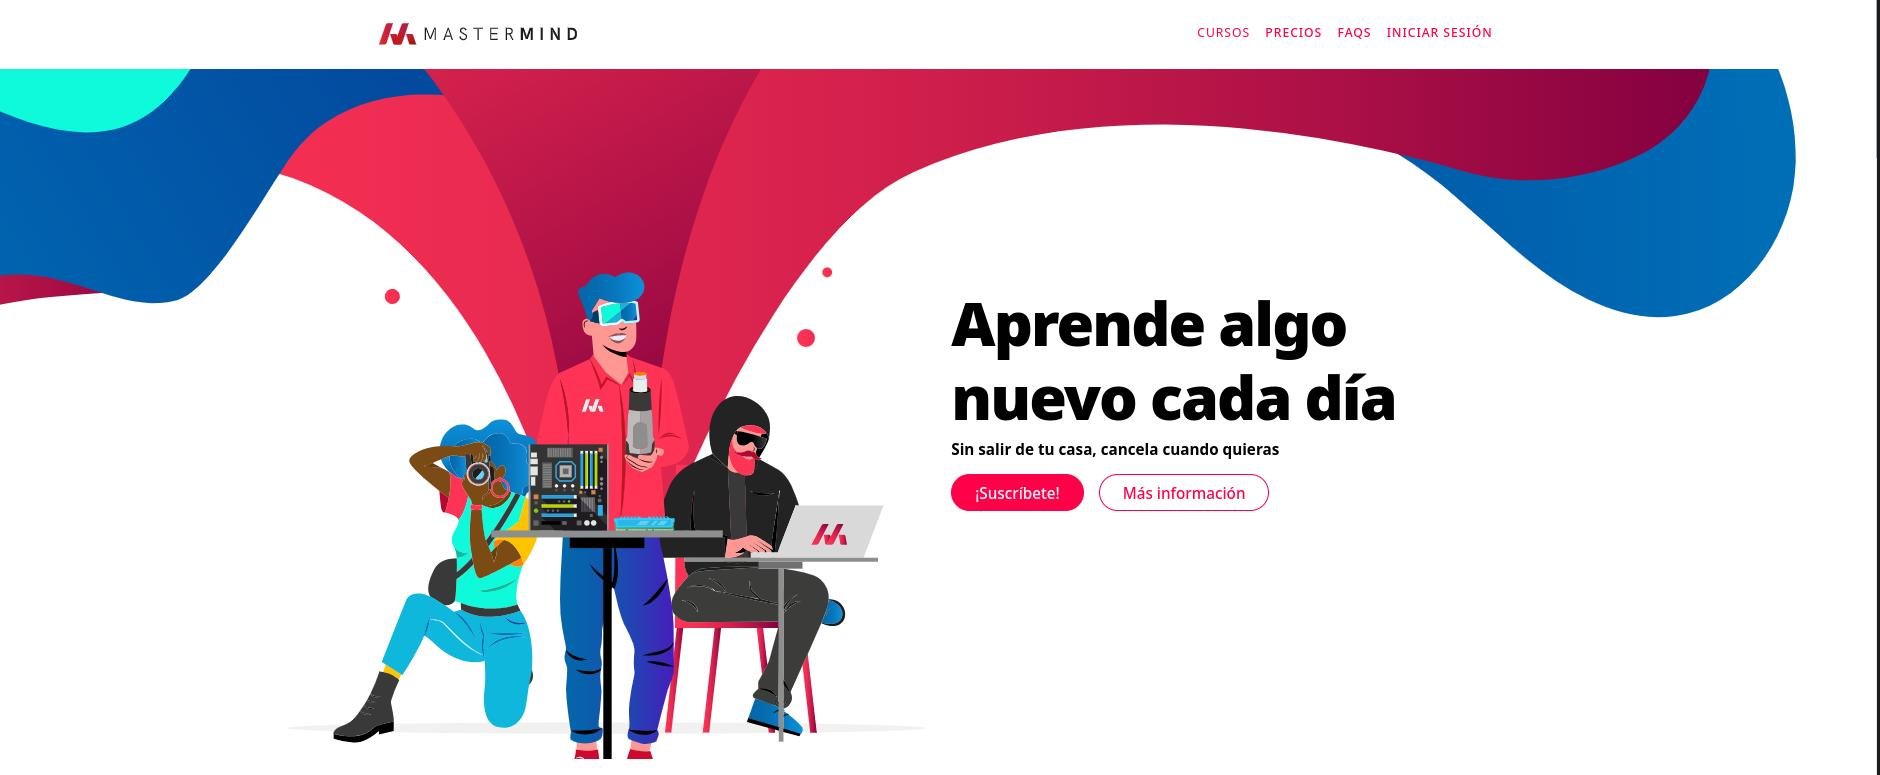
\includegraphics[width=\textwidth]{\prototipo}
		\caption{Prototipo de sitio web aplicando la ley de fitts}
	\end{figure}

	\subsubsection{Conclusión}

	El análisis de la página principal de VirusTotal utilizando la Ley de
	Fitts sugiere que la organización y el tamaño de los elementos clave
	en el sitio web ayudan a mejorar la eficiencia de uso, aunque
	siempre se puede optimizar el diseño para reducir aún más el tiempo
	de interacción y mejorar la precisión.

	%% References

	\nocite{*} % to include uncited references of .bib file

	\clearpage
	\bibliographystyle{ieeetr}

	% Generated from .bib file
	\bibliography{ref}
\end{document}
